\newcommand{\ssection}[1]{\addcontentsline{toc}{subsection}{#1, }
\subsection*{#1}%
}%

{\setbeamertemplate{footline}{\usebeamertemplate*{minimal footline}}%
\begin{frame}
    \frametitle{Outline}%
	\tableofcontents%
\end{frame}%
}%


\section{Introduction}%
\ssection{Molecular Electronics}
\begin{frame}
    \frametitle{Molecular Junction}
    \begin{figure}[!b] 
        \centering
        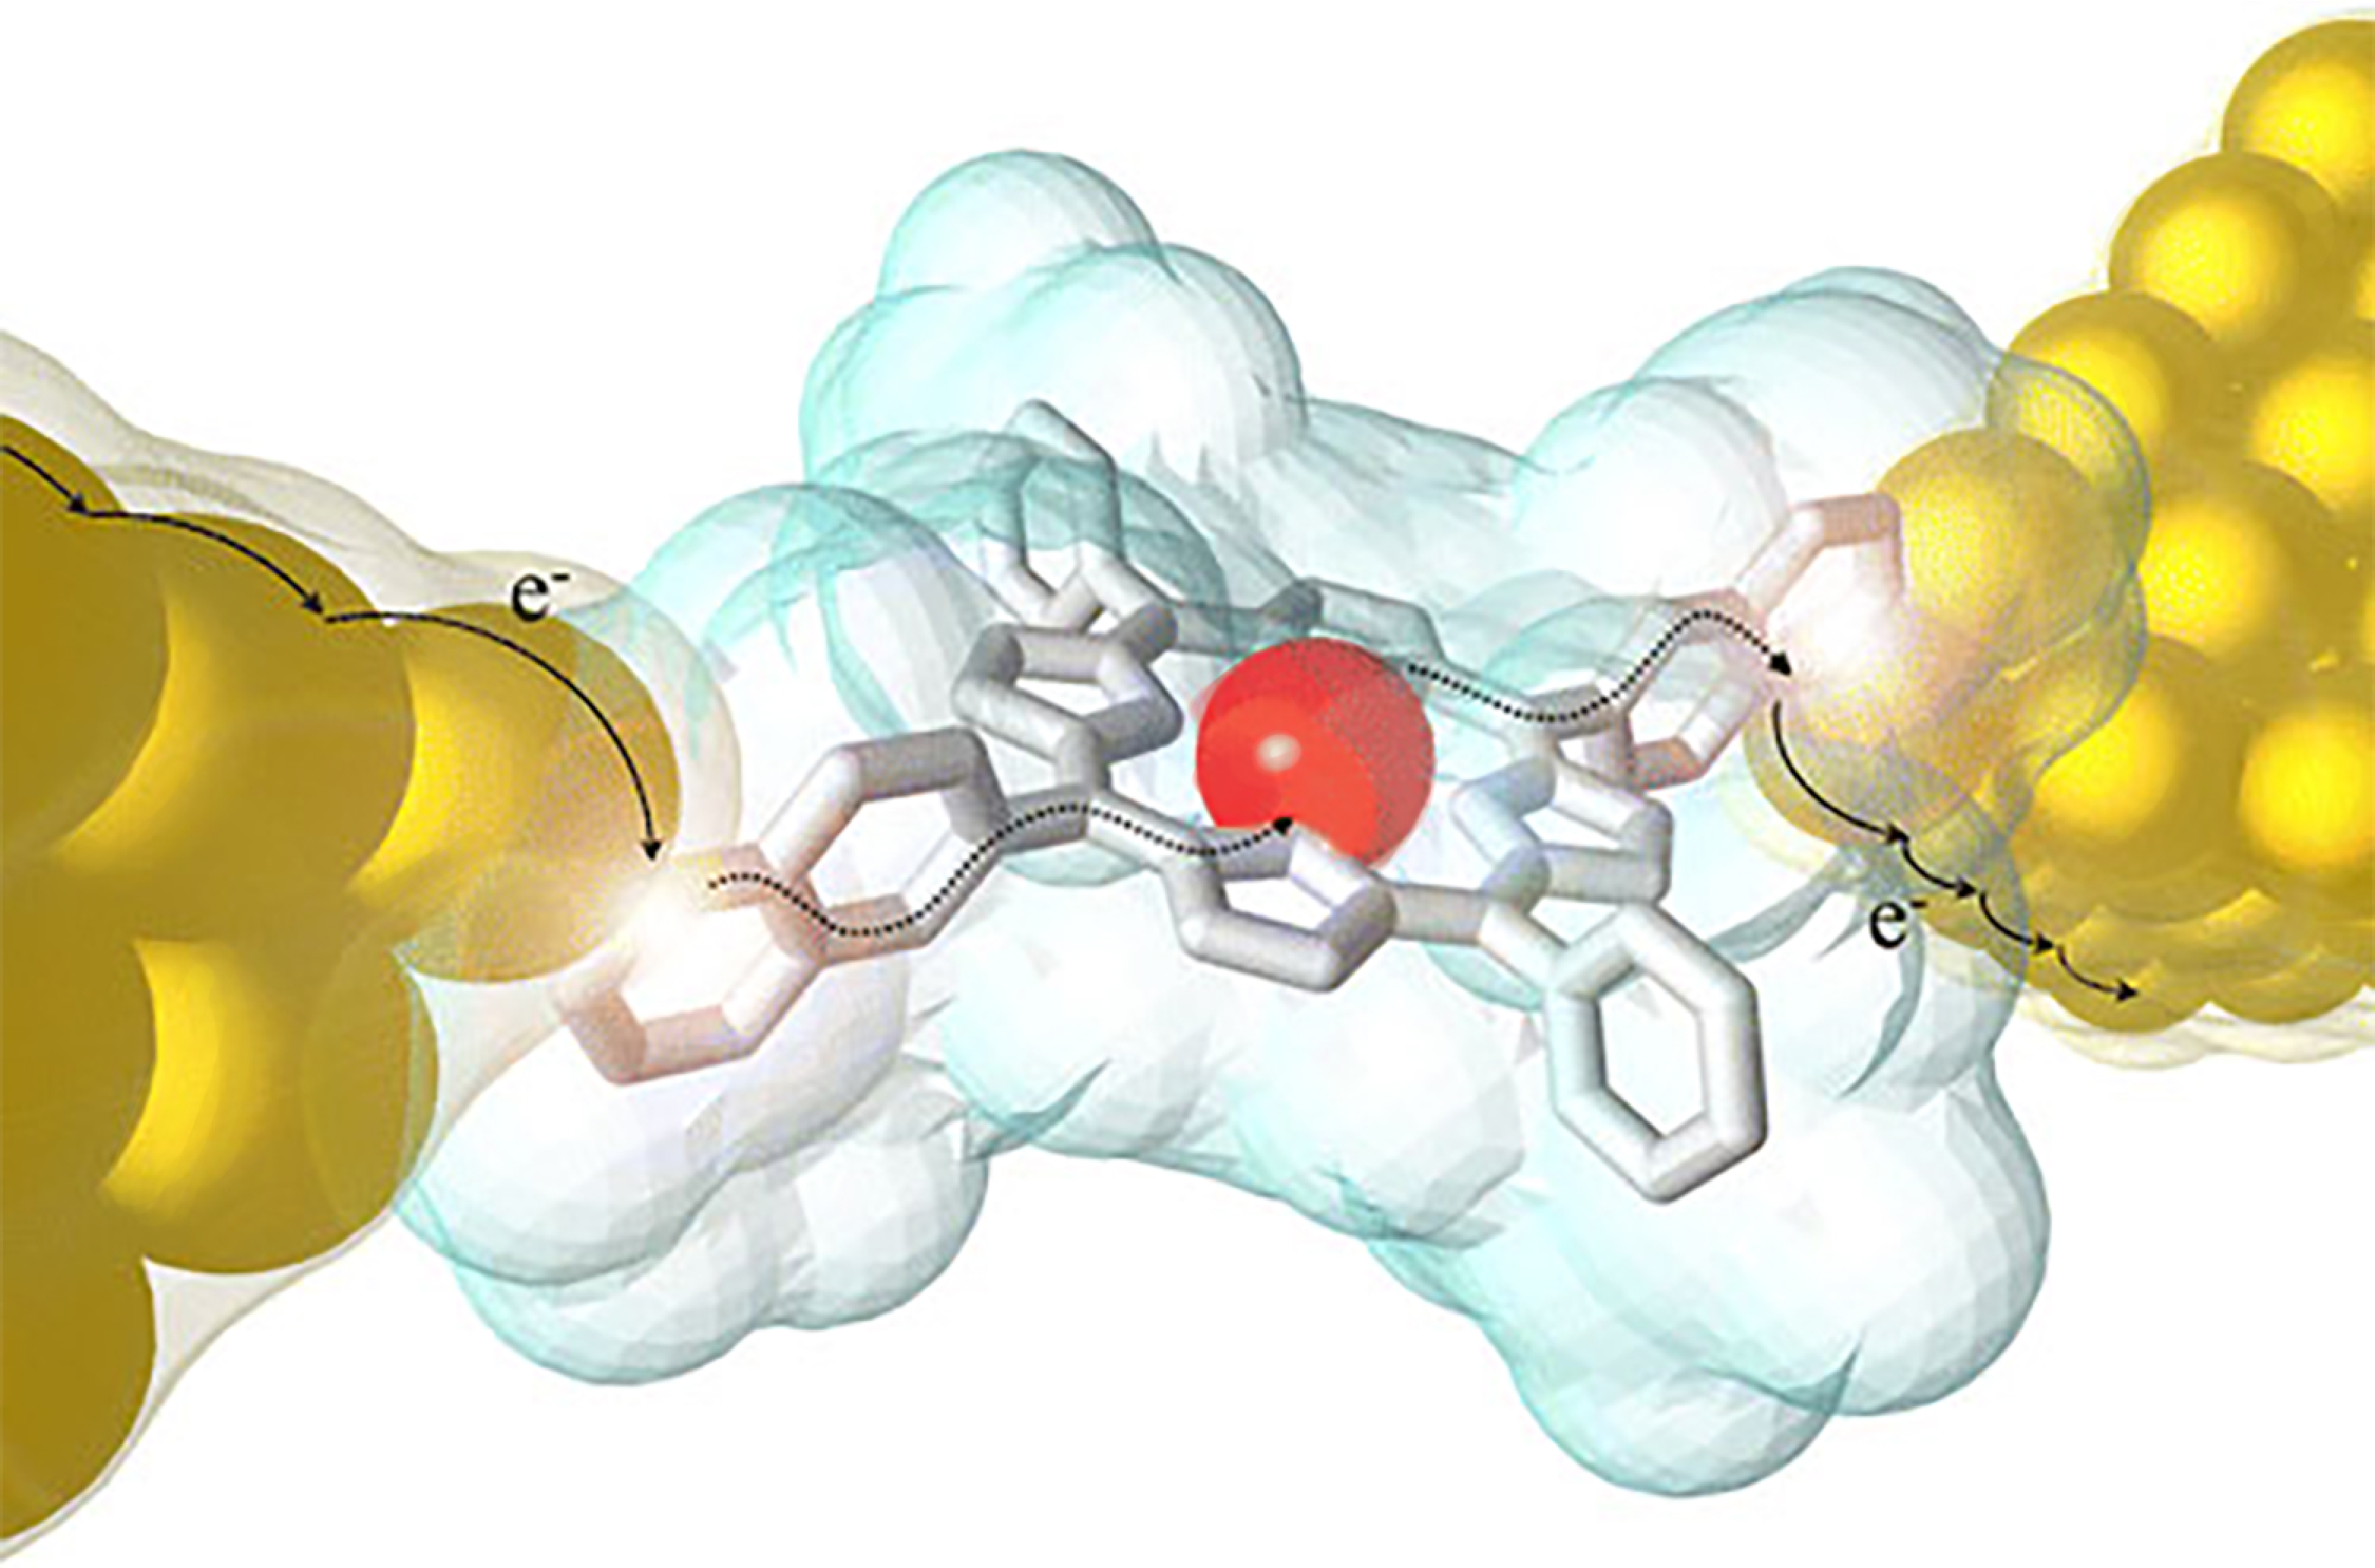
\includegraphics[height=0.5\textheight]{fig/junction.pdf}
        \caption{Artist impression of a  molecular junction. Via ~\citet{junction}.}
    \end{figure} 
\end{frame}%
\ssection{Green's Functions (Analogy)}
\begin{frame}
    \frametitle{Waves}
    \begin{figure}[!b] 
        \centering
        \includegraphics[height=0.5\textheight]{fig/wavepatterns.pdf}
        \caption{Interfering circular wave patterns (left) and fluorescent algae lightening up the wave crests (right).}
    \end{figure} 
\end{frame}%
\begin{frame}
    \frametitle{A music instrument.}
    \begin{figure}[!b] 
        \centering
        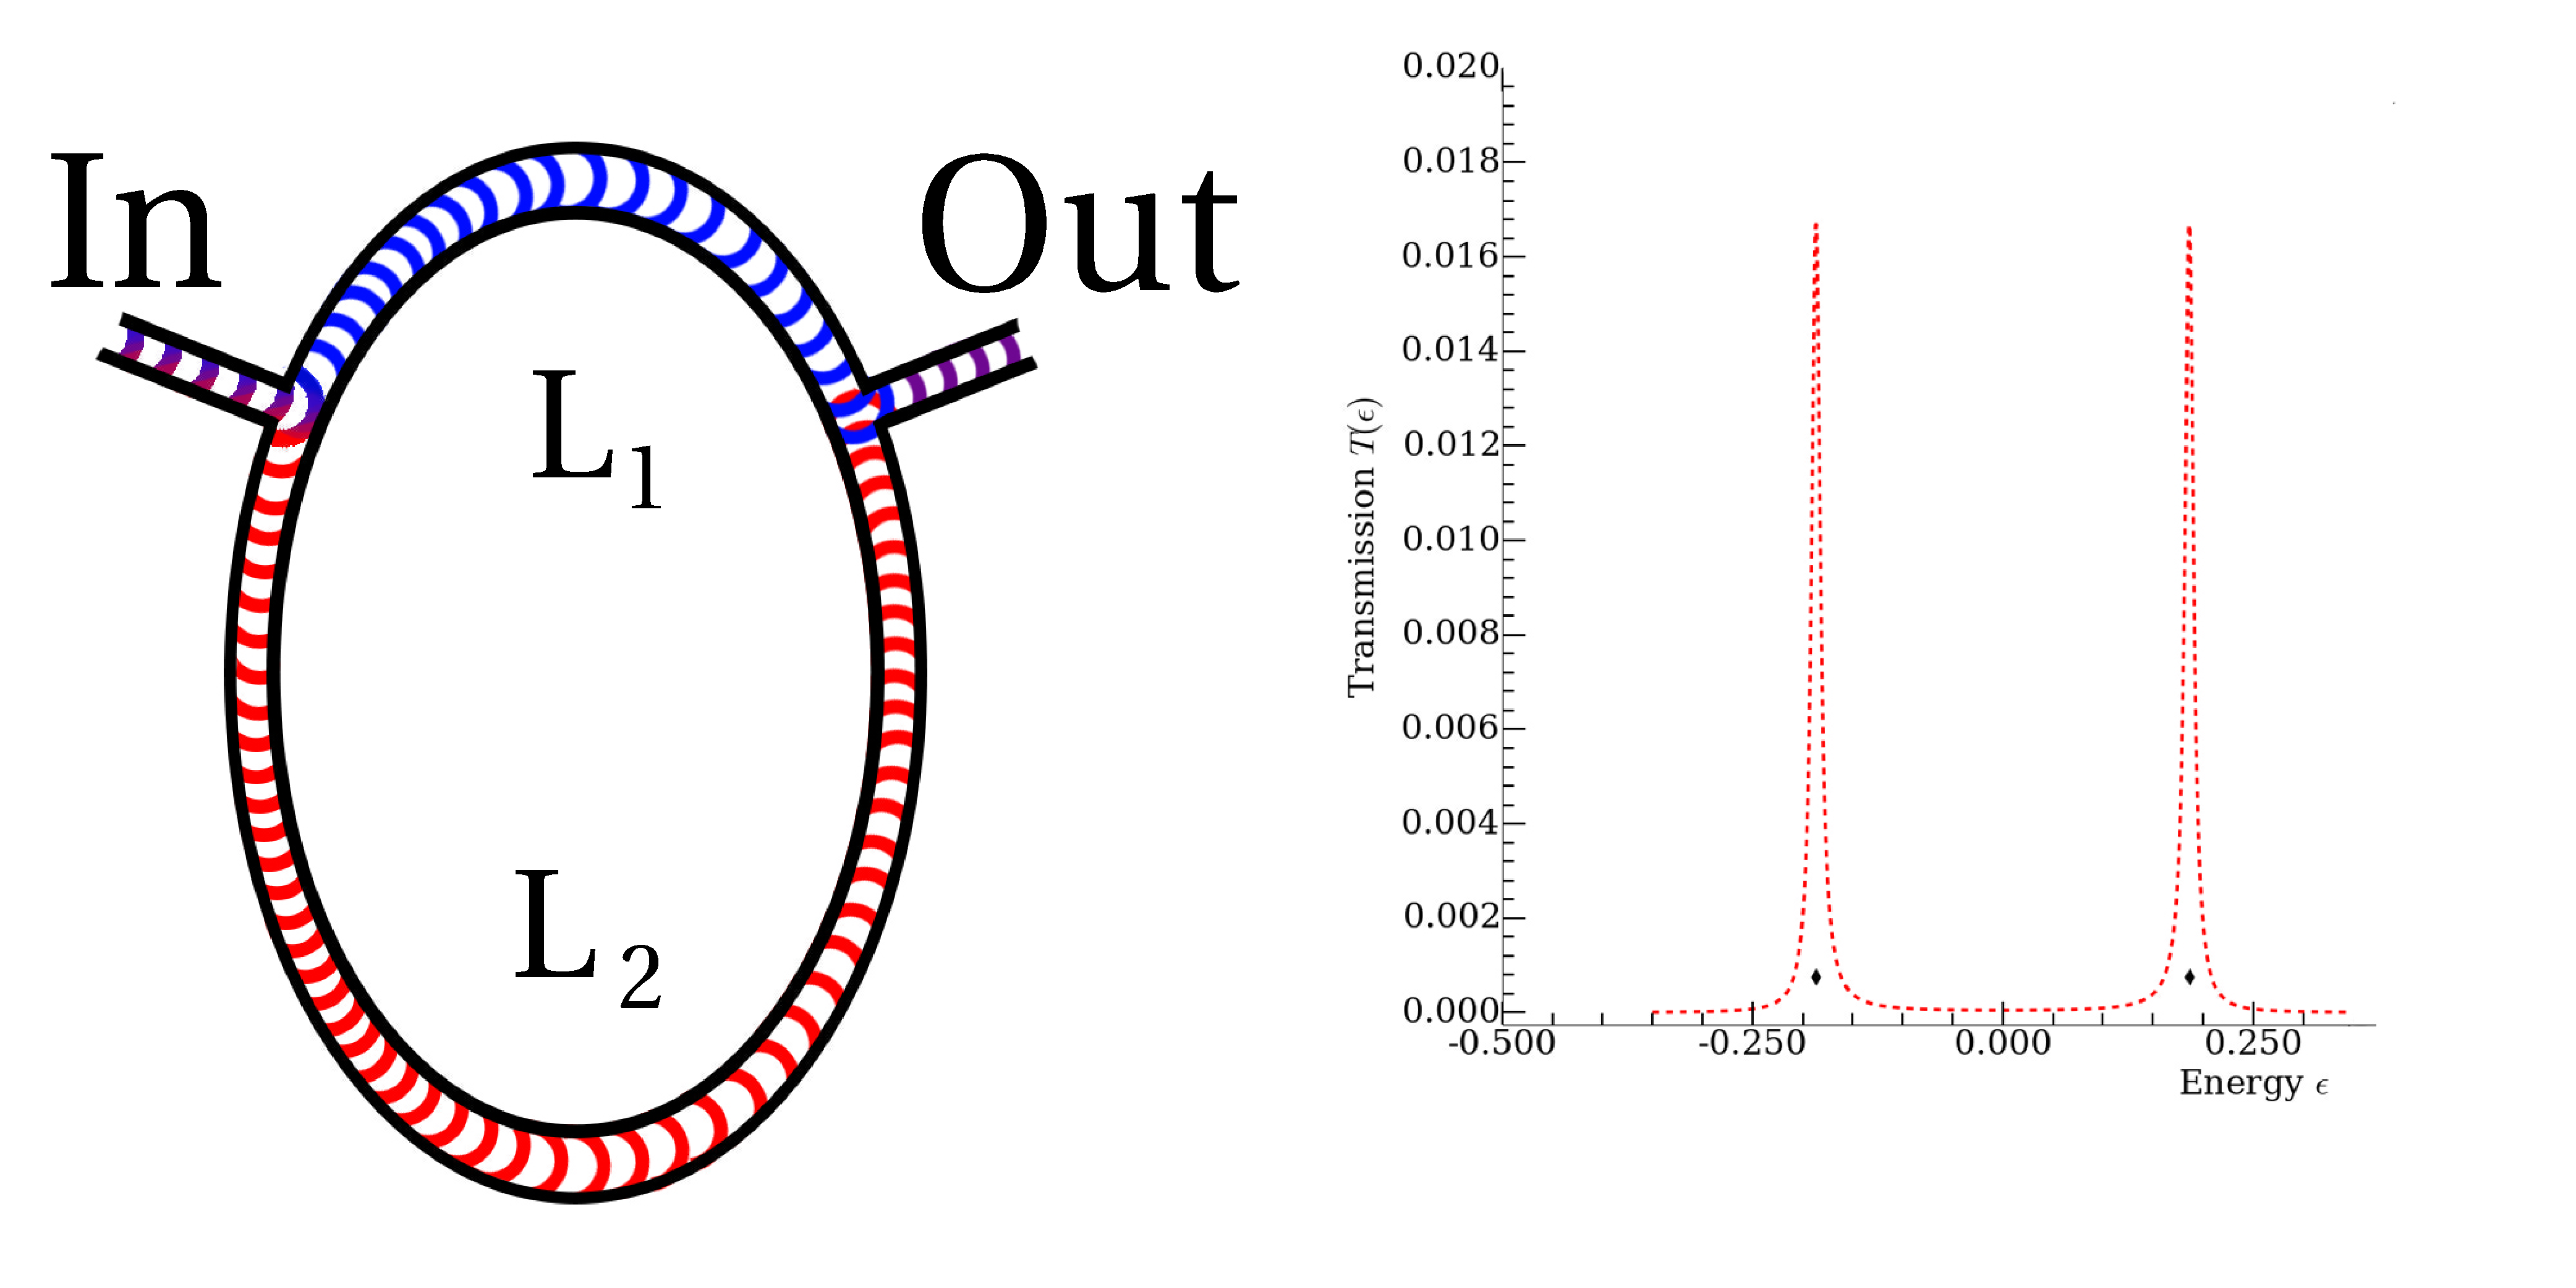
\includegraphics[height=0.5\textheight]{fig/acoustic.pdf}
        \caption{(left) Illustration of a instrument that would use interference. To the right, the notes or transmission peaks are shown.}
    \end{figure} 
\end{frame}%
\begin{frame}
    \frametitle{A music instrument.}
    \begin{figure}[!b] 
        \centering
        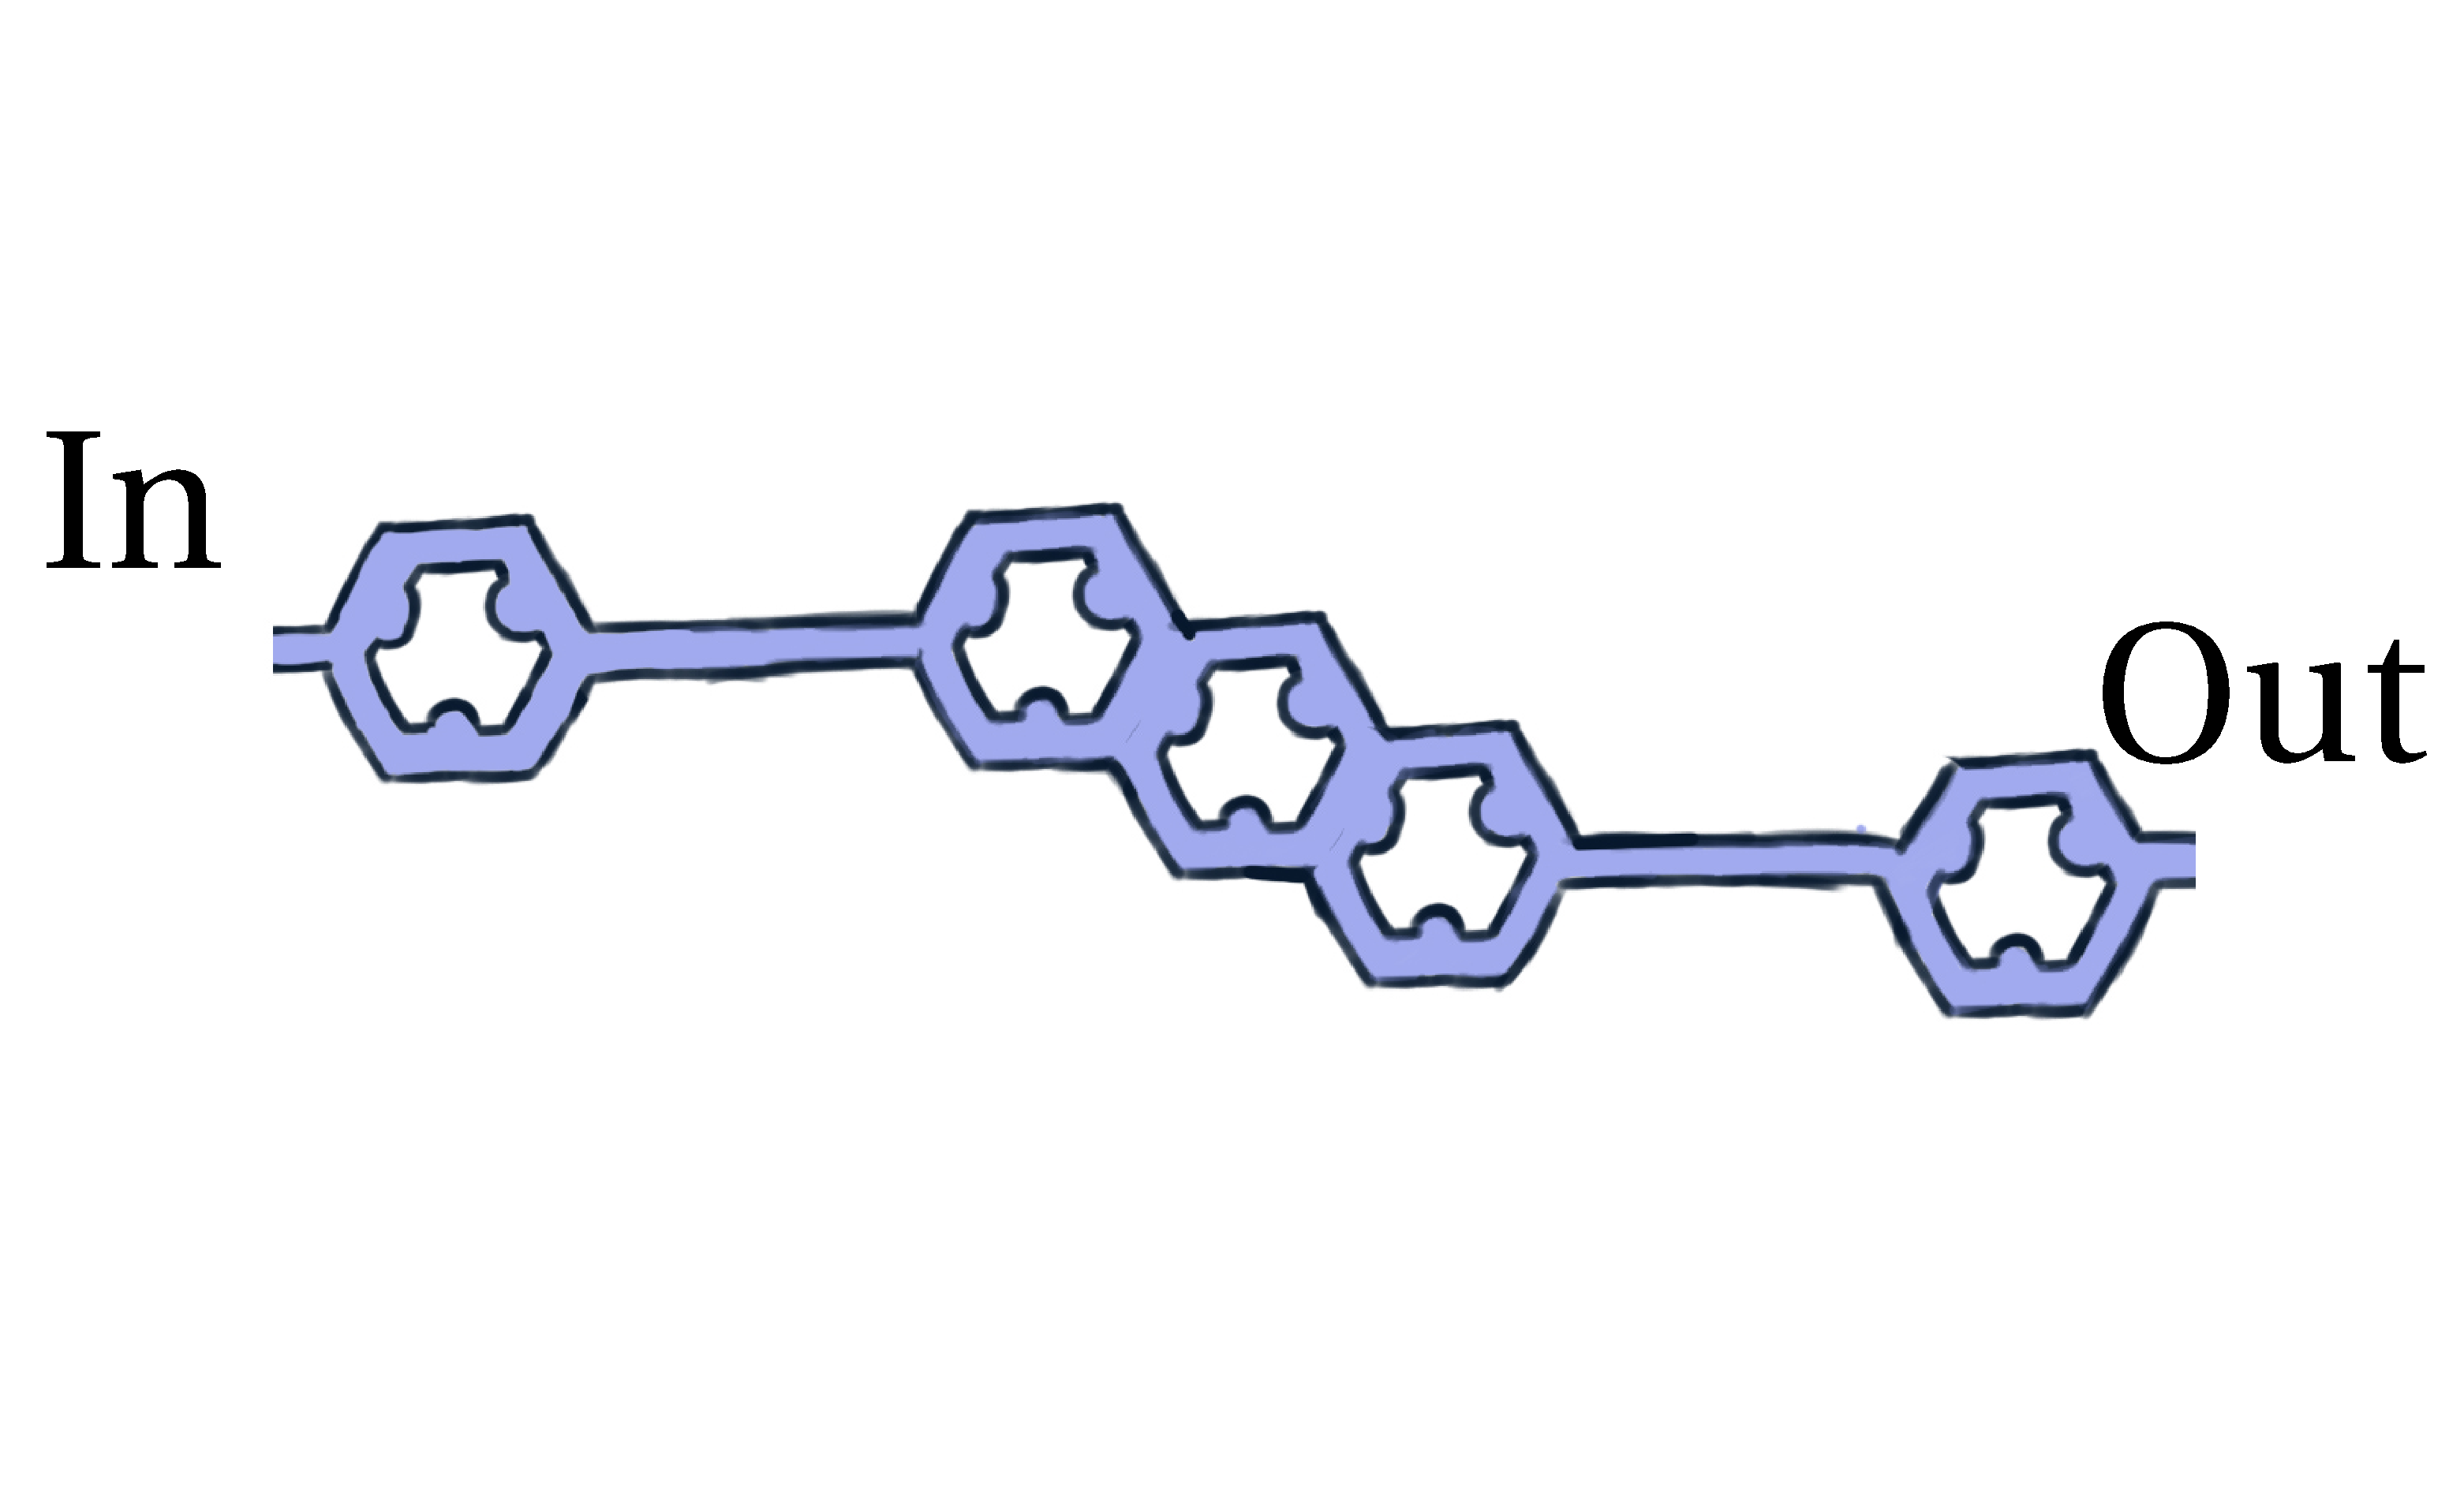
\includegraphics[height=0.5\textheight]{fig/molecule.pdf}
        \caption{The molecule displayed as a set of pipes to blow air through. Very complex, with many parts and lots of intersections.}
    \end{figure} 
\end{frame}%
\begin{frame}
    \frametitle{Flowing currents.}
    \begin{figure}[!b] 
        \centering
        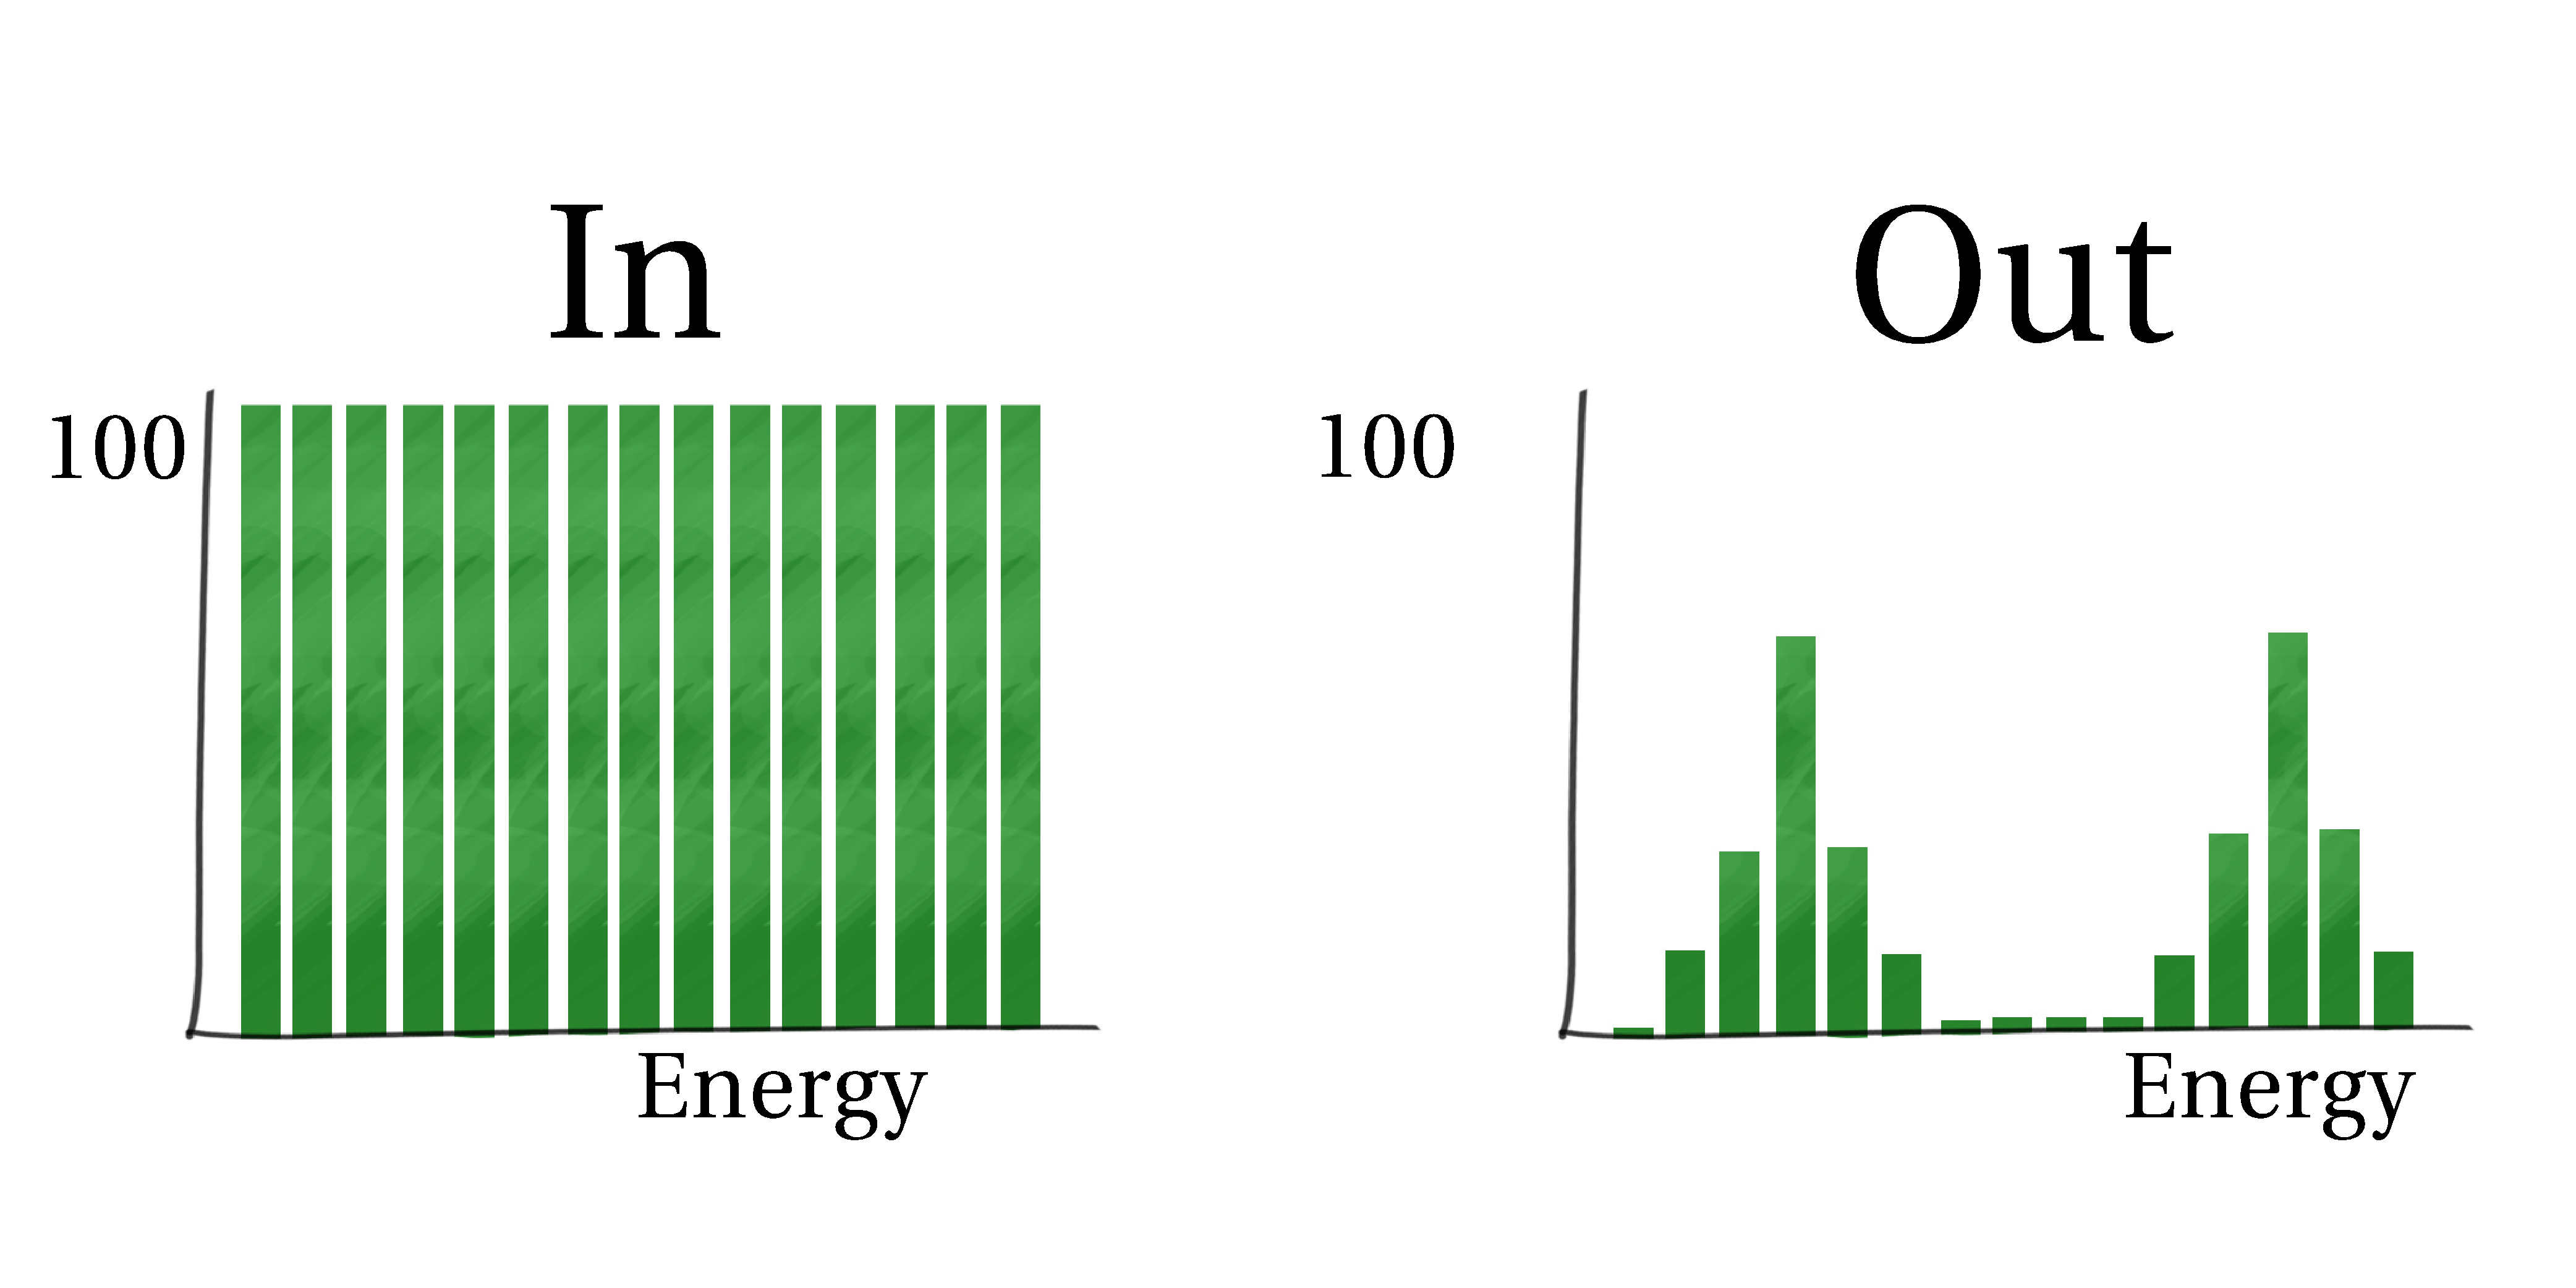
\includegraphics[height=0.5\textheight]{fig/current.pdf}
        \caption{To the left, we see the input-electrons, distributed at low-temperature. The right shows the electrons that pass the molecule - only those at the correct values.}
    \end{figure} 
\end{frame}%
\begin{frame}
    \frametitle{Current versus potential difference.}
    \begin{figure}[!b] 
        \centering
        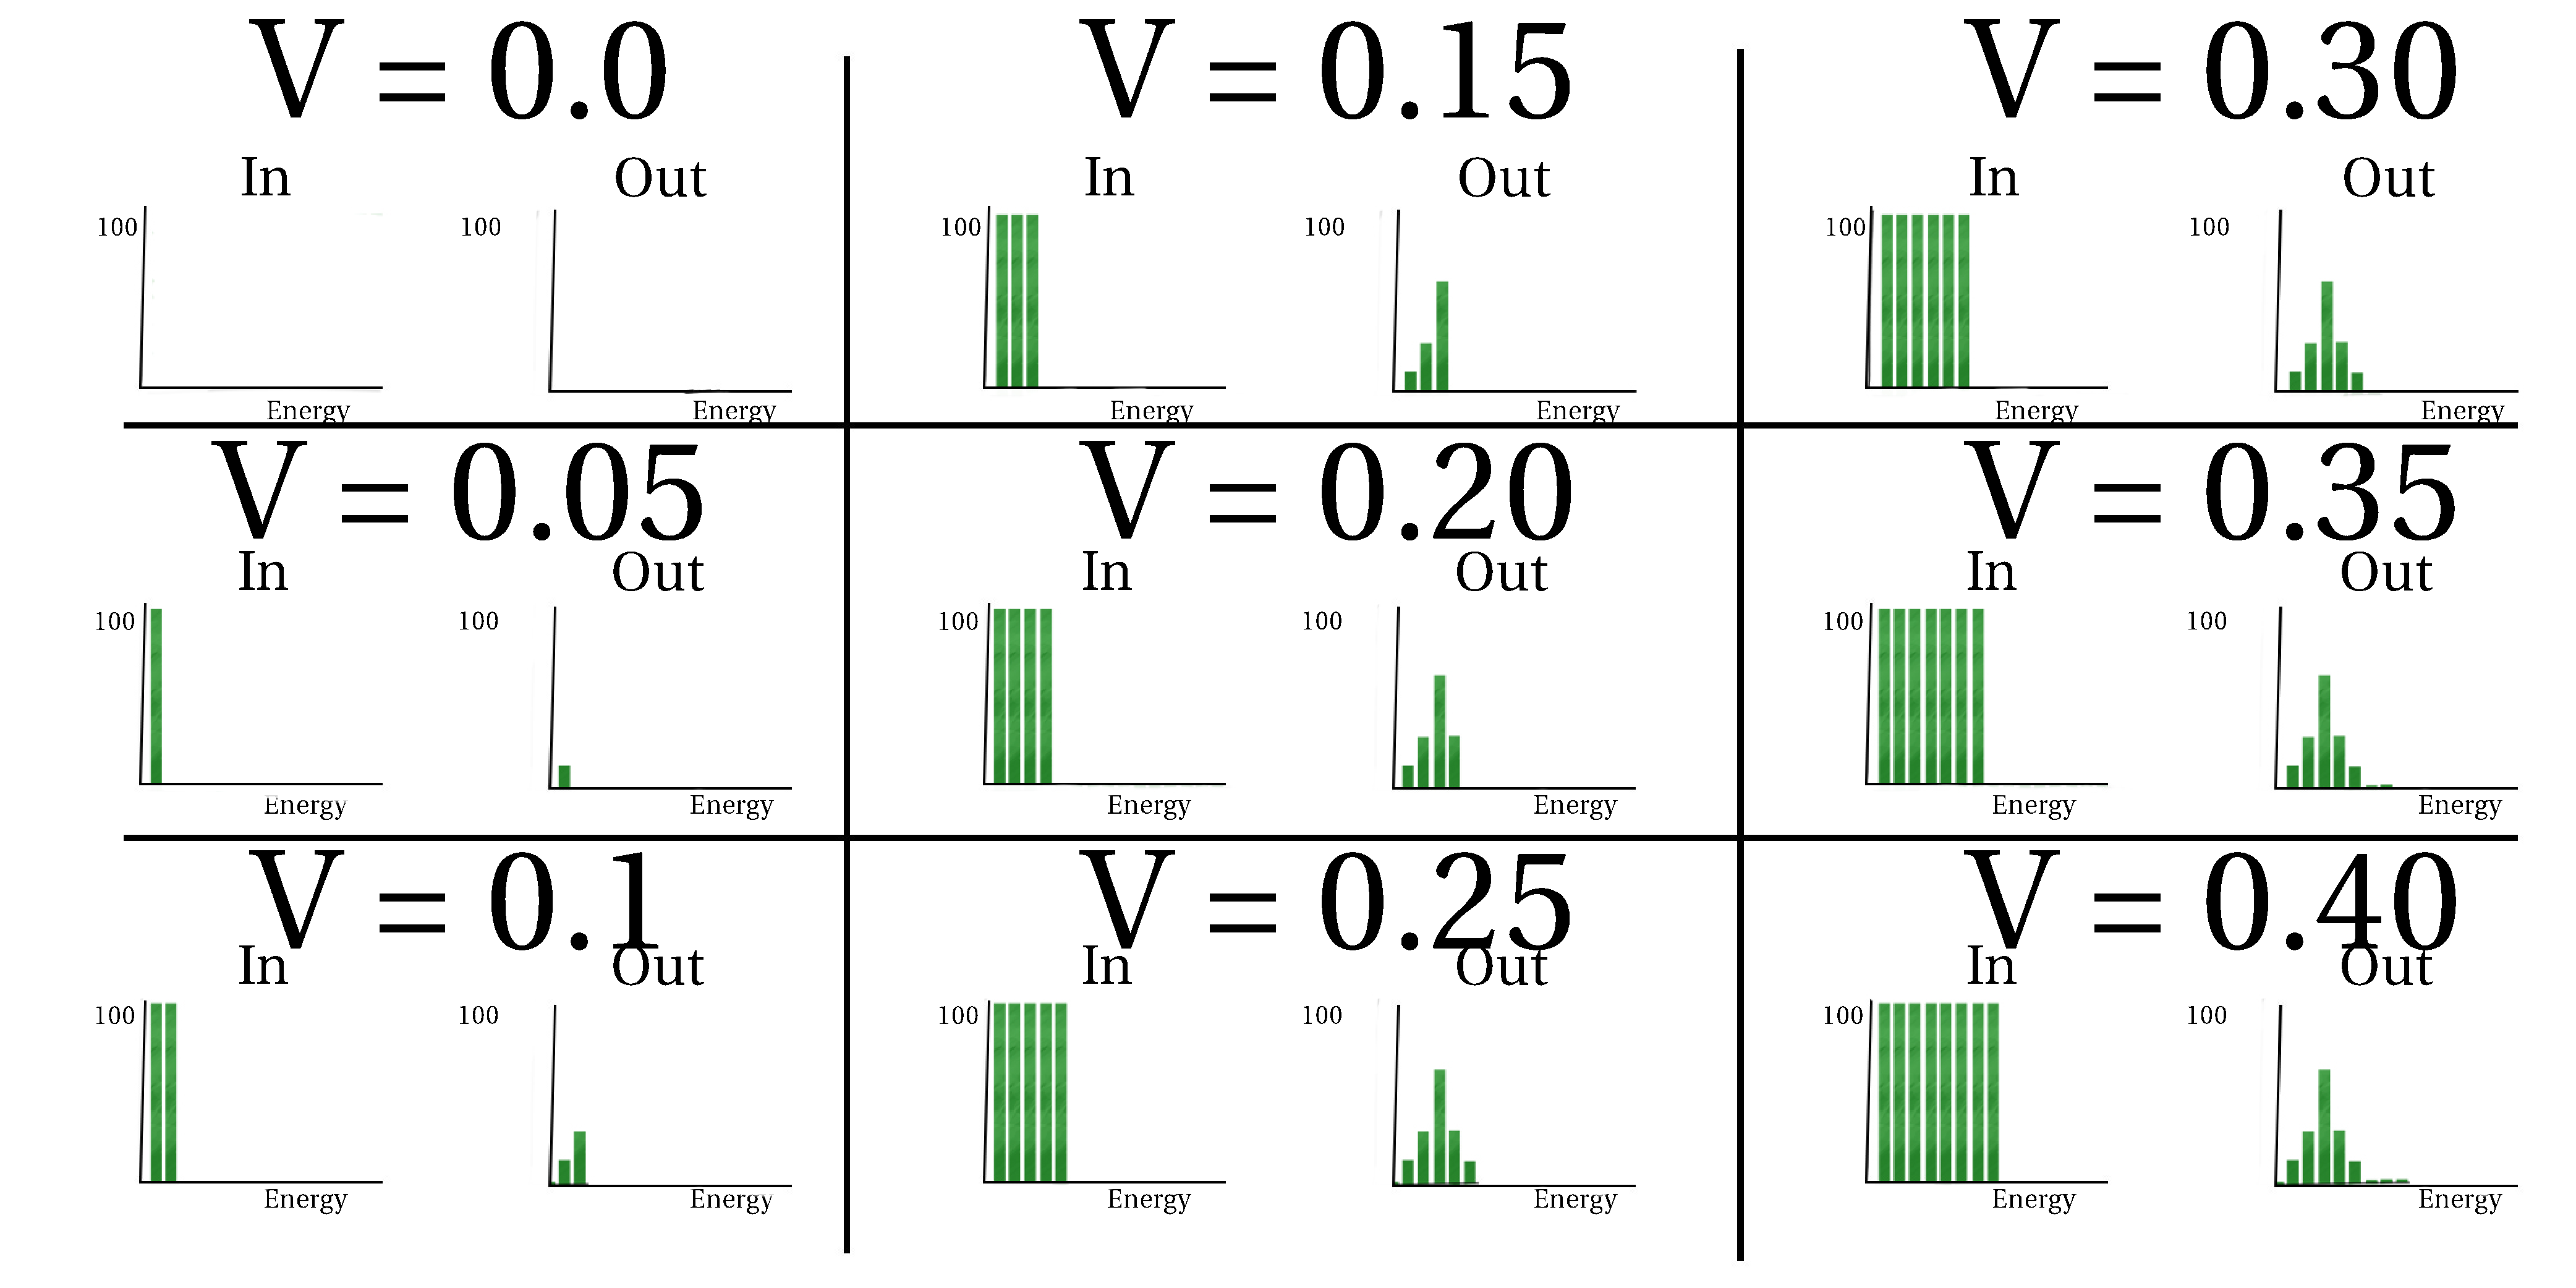
\includegraphics[width=\textwidth]{fig/current_calculation2.pdf}
        \caption{Image from the previous slide for various voltages.}
    \end{figure} 
\end{frame}%
\ssection{Summary}% 
\begin{frame}
    \frametitle{Summary.}
    \begin{itemize}
        \item Molecules are complicated.
        \item Molecules have 'notes' or so-called \emph{transmission peaks}.
        \item The \emph{Green's Function formalism} can calculate the transmission peaks.
        \item The transmission peaks determine the \emph{current}.
        \item The current is found by putting blocks of electrons through the transmission graph, and counting how many came out.
        \item Various things haven't been calculated yet.
    \end{itemize} 
\end{frame}%
\begin{frame}
    \frametitle{Next}
	\tableofcontents[currentsection,currentsubsection]
\end{frame}
\section{Theory}
\ssection{Single-Particle Green's Function}
\begin{frame}
    \frametitle{The Single-Particle Green's Function}
     \begin{itemize}
     \item A particle is created in state $i$ at time $t'$.
     \item The Green's function $G_{ij}(t,t')$.
     \item The probability it is found in state $j$ at time $t$.
     \item Green's Function contains the sum of all possible interactions
     \end{itemize}
    
    \begin{figure}[!b] 
        \centering
        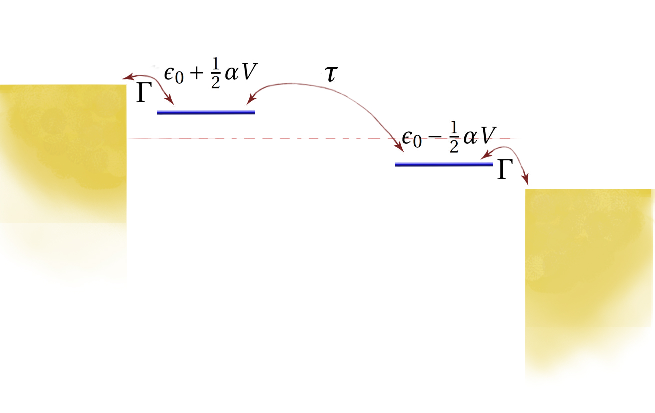
\includegraphics[height=0.5\textheight]{fig/non_interacting_schematics.pdf}
        \caption{Single-Particle Green's Function in a picture.}
    \end{figure} 
\end{frame} 
\begin{frame}
    \frametitle{Coulomb Interaction}
     \begin{itemize}
     \item Electrons carry charge $-e$.
     \item Electrons repulse.
     \item Interaction energy $U = \braket{\varphi_1 \left| V(r^\mu_1, r^\mu_2)\right|\varphi_2}$.
     \item Add to Green's Function?
     \end{itemize}
    
    \begin{figure}[!b] 
        \centering
        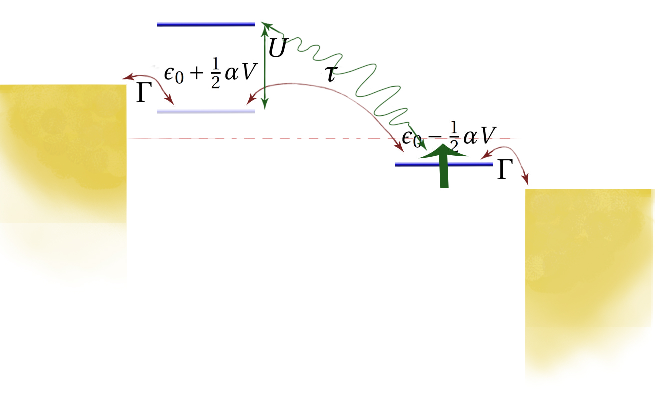
\includegraphics[height=0.5\textheight]{fig/interacting_schematics.pdf}
        \caption{Single-Particle Green's Function in a picture.}
    \end{figure} 
\end{frame}
\begin{frame}
    \frametitle{Many-Body Green's Function} 
    Denoted $\mathscr{G}(\epsilon)$.
    \begin{figure}[!b]  
        \begin{subfigure}{0.45\textwidth}\centering
            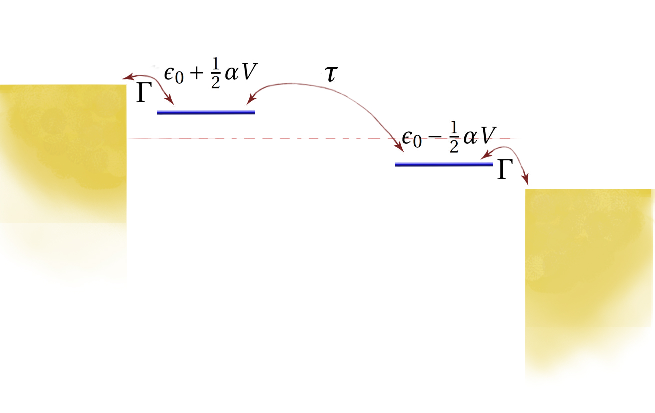
\includegraphics[clip=true,trim=0cm 1cm 0cm 0cm, width=0.65\textwidth]{fig/non_interacting_schematics.pdf}
            \caption{No electrons present.}
        \end{subfigure}~ 
        \begin{subfigure}{0.45\textwidth}\centering
            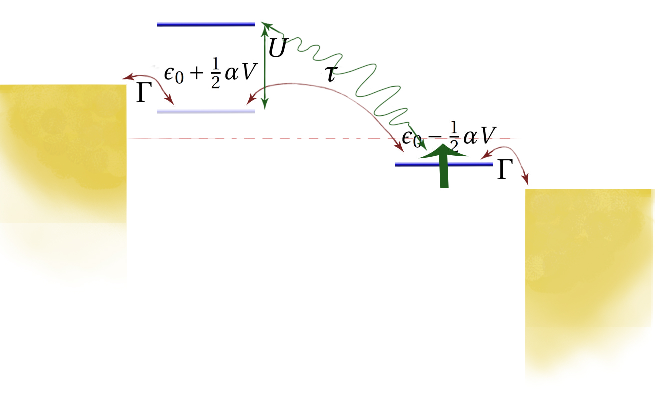
\includegraphics[clip=true,trim=0cm 1cm 0cm 0cm, width=0.65\textwidth]{fig/interacting_schematics.pdf}
            \caption{Electron present on the right.}
        \end{subfigure}
        
         
        \begin{subfigure}{0.45\textwidth}\centering
            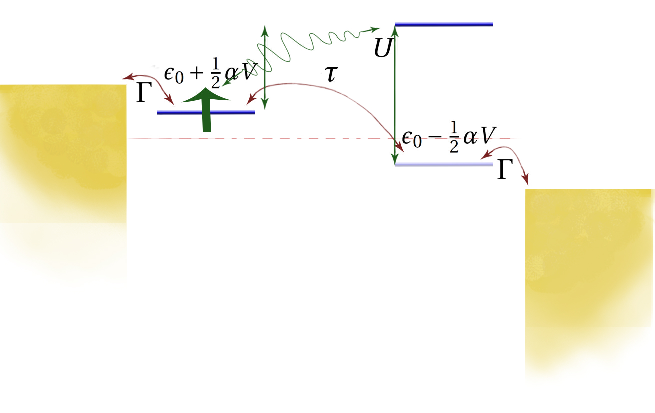
\includegraphics[clip=true,trim=0cm 1cm 0cm 0cm, width=0.65\textwidth]{fig/interacting_schematics2.pdf}
            \caption{Electron present on the left.}
        \end{subfigure}~ 
        \begin{subfigure}{0.45\textwidth}\centering
            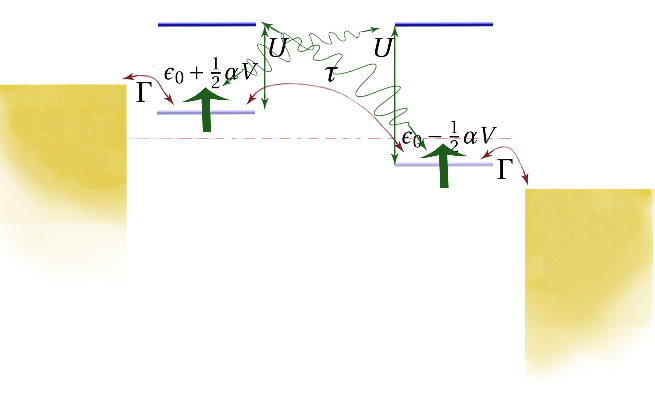
\includegraphics[clip=true,trim=0cm 1cm 0cm 0cm, width=0.75\textwidth]{fig/interacting_schematics3.pdf}
            \caption{Electron present on both the right and the left.}
        \end{subfigure}
        \caption{The many-body Green's Function is found as a weighted sum of single-particle Green's Functions.} 
    \end{figure} 
\end{frame}
\ssection{Many-body Green's Function}
\ssection{Density Matrix}
\ssection{Two site model}
\begin{frame}
    \frametitle{Next}
	\tableofcontents[currentsection,currentsubsection]
\end{frame}
\section{Results}
\ssection{Transmission}
\ssection{Coulomb Diamonds}
\ssection{Experimental Fit}
\ssection{Non-equilibrium density Matrix}
\begin{frame}
    \frametitle{Next}
	\tableofcontents[currentsection,currentsubsection]
\end{frame}
\section{Conclusions}
\ssection{Summary}
\ssection{Discussion}
\ssection{Future Outlook}